\subsection{UC4 - Seleziona quota disco}
\label{UC4}
\begin{figure}[H]
    \centering
    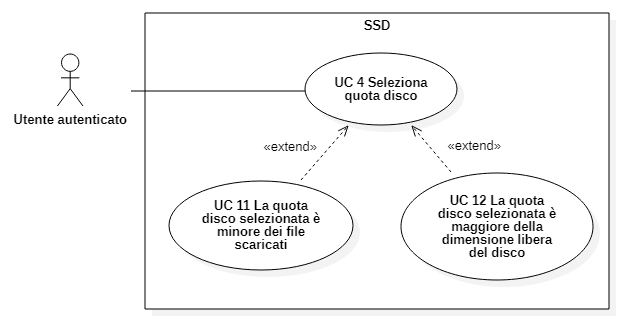
\includegraphics[scale = 0.7]{components/img/UC4.png}
    \caption{UC4 - Seleziona quota disco}
\end{figure}
\begin{itemize}
\item \textbf{Attore Primario:} Utente autenticato;
\item \textbf{Precondizione:} L'utente vuole cambiare la dimensione disco riservata, lato client, per le iterazioni con \glo{Zextras Drive};
\item \textbf{Postcondizione:} L'utente ha cambiato lo spazio disco riservato per l'applicativo;
\item \textbf{Scenario principale:}
    \begin{enumerate}
    \item L'utente necessita di cambiare lo spazio disco dedicato;
        \begin{itemize}
        \item L'utente ha poco spazio nel disco e vuole ridurre lo spazio dedicato per le iterazioni con \glo{Zextras Drive};
        \item L'utente ha abbastanza spazio disponibile da voler aumentare lo spazio disco dedicato per le iterazioni con \glo{Zextras Drive};
        \end{itemize}
    \item L'utente ha cambiato lo spazio disco dedicato.
    \end{enumerate}
\item \textbf{Estensioni:}
    \begin{itemize}
        \item La quota disco selezionata è minore dei file scaricati (UC11 \S{}\ref{UC11});
        \item La quota disco selezionata è maggiore della dimensione libera del disco (UC12 \S{}\ref{UC12}).
    \end{itemize}
\end{itemize}